\documentclass{jsarticle}
\title{講義ノート第7回}
\author{}
\date{}


\usepackage[top=30truemm,bottom=30truemm,left=25truemm,right=25truemm]{geometry}

\usepackage{ascmac}

\usepackage{amsmath}

\usepackage[dvips]{graphicx}

\usepackage{ulem}

\parindent = 0pt

\begin{document}
\maketitle

\section{静電場}

\setcounter{subsection}{12}

\subsection{導体}
内部を電荷が自由に移動できる物質を導体という.一方,内部で電荷が自由に移動できない物質を絶縁体という.以下に導体と絶縁体の例を挙げる. \\
導体 \\
金属,黒鉛,イオン溶液 \\
抵抗率:$10^{-8}~10^{-6} \Omega m$ \\
\\
絶縁体 \\
ゴム,ガラス,大部分のプラスチック,木,空気 \\
抵抗率:$10^{10} \Omega m$ \\

\begin{figure}[htbp]
 \begin{center}
  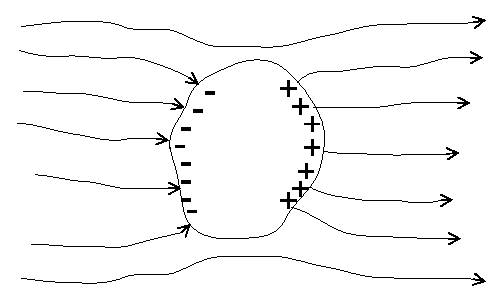
\includegraphics[width=80mm]{7.1.eps}
 \end{center}
 \caption{}
 \label{fig:one}
\end{figure}
導体内では電荷が自由に動くことができる.そのような電荷を誘導電荷と呼ぶ.導体を一様な電場の中に置くと,誘導電荷は外部の電場によって導体内を
移動して,静的状態となる.静的状態では外部電場と,誘導電荷によって導体内につくりだされる電場は重ね合わせて完全に打ち消しあう.したがって静的状態にある導体内では${\bf E}={\bf 0}$が成り立つ.Gaussの法則(微分形)より導体内の電荷密度は$\rho = \varepsilon_0 {\rm div}{\bf E} = 0$となり,電荷は導体の表面にだけ分布する.したがって11節の例から,導体は等電位であることが分かる.特に導体表面は等電位面であり,${\bf E} \perp \mbox{導体表面}$ となる. \\
\\
{\bf 例:静電遮蔽} \\
\begin{figure}[htbp]
 \begin{center}
  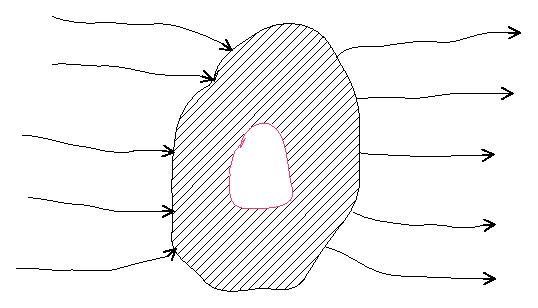
\includegraphics[width=80mm]{7.2.eps}
 \end{center}
 \caption{}
 \label{fig:two}
\end{figure}
図のような中空導体を考える.中空領域では電荷密度が0とすると,中空領域と導体の境界は等電位面となる.その電位を$\phi_0$とする.ここで中空領域では$\rho = 0$であるから,Poisson方程式より$\Delta \phi = - \frac{\rho}{\varepsilon_0}=0$ 解は容易に$\phi = \phi_0$ と分かる.中空領域の電場は${\bf E}=-{\rm grad}\phi_0 = {\bf 0}$ このように導体に囲まれた中空領域ではいたるところ電場は{\bf 0}である.\footnote{間違えて「電場は存在しない」などと書かないようにしたい.}このような効果を{\bf 静電遮蔽}という. \\
\\
{\bf 例:電気鏡映} \\
\begin{figure}[htbp]
 \begin{center}
  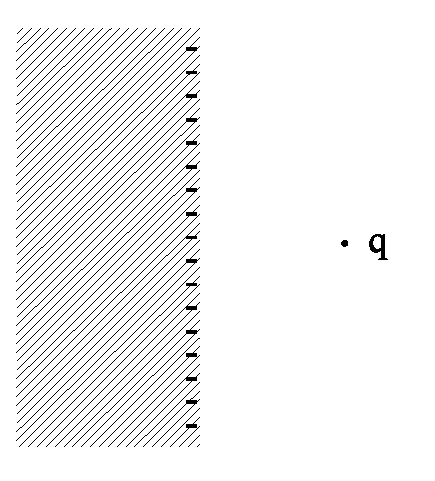
\includegraphics[width=50mm]{7.3.eps}
 \end{center}
 \caption{}
 \label{fig:three}
\end{figure}
\begin{figure}[htbp]
 \begin{center}
  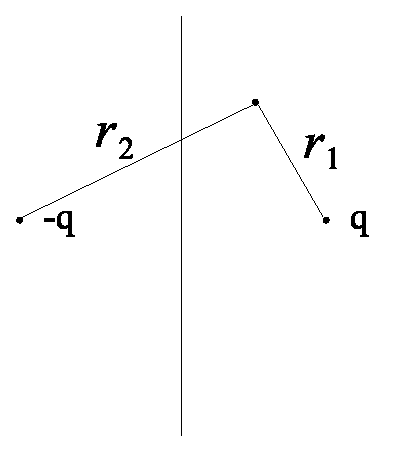
\includegraphics[width=50mm]{7.4.eps}
 \end{center}
 \caption{}
 \label{fig:four}
\end{figure}
導体表面至るところで$\phi=0$とする.\\
いま,導体を無いものと仮定し,代わりに導体表面があったx=0に関して対称な位置に電荷$-q$の電荷があると仮想する.これを仮想電荷という.すると電位は以下のように書ける.
\begin{eqnarray*}
\phi = \frac{q}{4 \pi \varepsilon_0} \left( \frac{1}{r_1} - \frac{1}{r_2} \right)
\end{eqnarray*}
ここで,この静電ポテンシャルには以下が成立する.
\begin{equation*}
\phi =\left \{
\begin{array}{l}
0 \quad (x=0)\\
0 \quad (x \to + \infty)
\end{array}
\right.
\end{equation*}
ここで$x>0$の領域に限って話を進めると,もとの問題のPoisson方程式と,境界条件を満たすので,解の一意性からこれはもとの問題の電位を与えていると結論してよい. \\
電荷は距離$2l$離れた自身の電気鏡映からの引力と等しい力を受ける. \\
\begin{figure}[htbp]
 \begin{center}
  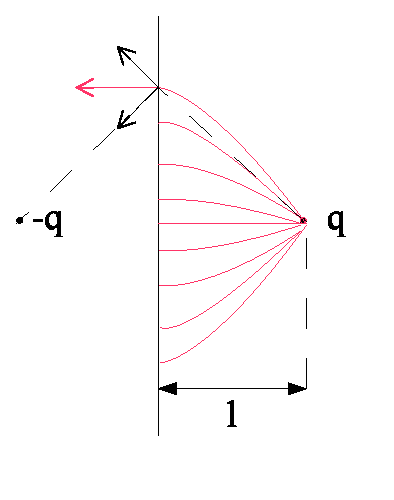
\includegraphics[width=50mm]{7.5.eps}
 \end{center}
 \caption{}
 \label{fig:five}
\end{figure}
\newpage
\section{定常電流と静磁場}
\subsection{電荷保存と連続の式}
ある時刻tに点${\bf r}$近傍の微小領域に,電荷$q_i$が速度${\bf v_i}$(i=1,2,...N)をもって存在する状況を考える.
すると点${\bf r}$の電荷密度$[Cm^{-3}]$は,微小領域を物理的に意味をもつ程度に小さくしていくという極限を$''V \to 0''$,と表すことにより,
\begin{eqnarray*}
\rho({\bf r},t) = \lim_{''V \to 0''} \frac{\sum_{i=1}^{N}q_i}{V}
\end{eqnarray*}
ここで{\bf 単位時間あたりに単位断面積を通過する電荷}を表すベクトル量として{\bf 電流密度}を以下のように定義する.
\begin{itembox}[c]{電流密度}
\begin{eqnarray}
{\bf i}({\bf r},t) = \lim_{''V \to 0''} \frac{\sum_{i=1}^{N}q_i{\bf v}_i}{V}
\end{eqnarray}
単位は$[Cms^{-1}m^{-3}]=[Cm^{-2}s^{-1}]=[Am^{-2}]$である. \\
電流密度はベクトル場をなす.
\end{itembox}
電流密度に関する保存則を導出してみる. \\
ある閉領域Vを仮定する.電流密度のVの表面にわたる積分は上の定義から,単位時間あたりにVの表面を通過する電荷となる.Vの表面を内側から外側に貫く方向を正とすると,これはV内の全電荷の時間変化率に$-$を掛けたものに等しくなる.したがって \\
\begin{eqnarray*}
\int_{\partial V}^{}{\bf i} \cdot {\bf dS} &=& - \frac{d}{dt} \int_{v}^{} \rho({\bf r},t) dV \\
&=& - \int_{V}^{} \frac{\partial \rho({\bf r},t)}{\partial t} dV
\end{eqnarray*}
さてここでGaussの定理を用いると,面積分を体積積分に書き換えることができる.つまり,
\begin{eqnarray*}
\int_{\partial V}^{}{\bf i} \cdot {\bf dS} = \int_{V}^{} {\rm div}{\bf i}\, dV
\end{eqnarray*}
合わせて
\begin{eqnarray*}
\int_{V}^{} \left( \frac{\partial \rho}{\partial t} + {\rm div}{bf i} \right) dV = 0
\end{eqnarray*}
これがどんな領域でも成り立つから以下の保存則が成り立つ.
\begin{itembox}[c]{連続の式}
\begin{eqnarray}
\frac{\partial \rho}{\partial t} + {\rm div}\,{\bf i} = 0
\end{eqnarray}
これは電荷が保存されることを意味している. \\
また,この式は流体に対して成り立つ一般的な式である.
\end{itembox}
特に定常状態では電荷密度の時間変化が0であるから$\frac{\partial \rho}{\partial t}=0$より${\rm div}\,{\bf i}=0$
\\
\begin{itembox}[c]{Ohmの法則}
$|{\bf E}|$が大きくなく等方的な物質では近似的に
\begin{eqnarray}
{\bf i} = \sigma {\bf E} \Leftrightarrow {\bf E} = \sigma^{-1} {\bf i}
\end{eqnarray}
$\sigma$:伝導率,$\sigma^{-1}$:抵抗率
\end{itembox}
{\bf 例} \\
\begin{figure}[htbp]
 \begin{center}
  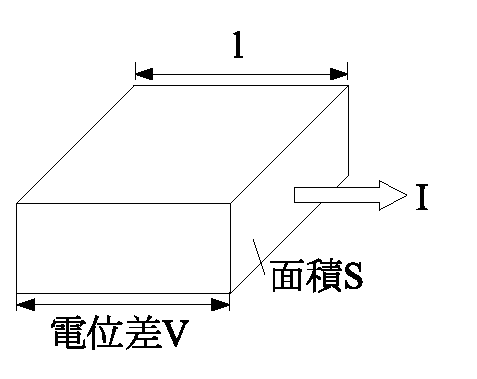
\includegraphics[width=50mm]{7.6.eps}
 \end{center}
 \caption{}
 \label{fig:six}
\end{figure}
\begin{eqnarray*}
I = S |{\bf i}| \\
V = l |{\bf E}|
\end{eqnarray*}
であるから抵抗は
\begin{eqnarray*}
R=\frac{V}{I} \cdot \frac{ l |{\bf E}|}{S |{\bf i}|} = \frac{l}{S}\sigma^{-1}
\end{eqnarray*}
電場${\bf E}$のもとで電流密度${\bf i}$が生じているとき,電場のする仕事率を体積で割ったものは,
\begin{eqnarray*}
\lim_{V \to 0} \frac{ \sum q_i {\bf E}  \cdot {\bf v}_i}{V} = {\bf E} \cdot {\bf i} = \sigma |{\bf E}|^2
\end{eqnarray*}
これはジュール熱や光となって散逸される.
\end{document}

